%%
%% This is file `tikzposter-template.tex',
%% generated with the docstrip utility.
%%
%% The original source files were:
%%
%% tikzposter.dtx  (with options: `tikzposter-template.tex')
%%
%% This is a generated file.
%%
%% Copyright (C) 2014 by Pascal Richter, Elena Botoeva, Richard Barnard, and Dirk Surmann
%%
%% This file may be distributed and/or modified under the
%% conditions of the LaTeX Project Public License, either
%% version 2.0 of this license or (at your option) any later
%% version. The latest version of this license is in:
%%
%% http://www.latex-project.org/lppl.txt
%%
%% and version 2.0 or later is part of all distributions of
%% LaTeX version 2013/12/01 or later.
%%


\documentclass{tikzposter} %Options for format can be included here

\usepackage{todonotes}

\usepackage[tikz]{bclogo}
\usepackage{lipsum}
\usepackage{amsmath}

\usepackage{booktabs}
\usepackage{longtable}
\usepackage[absolute]{textpos}
\usepackage[it]{subfigure}
\usepackage{graphicx}
\usepackage{cmbright}
%\usepackage[default]{cantarell}
%\usepackage{avant}
%\usepackage[math]{iwona}
\usepackage[math]{kurier}
\usepackage[T1]{fontenc}


%% add your packages here
\usepackage{hyperref}
% for random text
\usepackage{lipsum}
\usepackage[english]{babel}
\usepackage[pangram]{blindtext}

\colorlet{backgroundcolor}{blue!10}

 % Title, Author, Institute
\title{Group Outlying Aspects Mining}
\author{Shaoni Wang$^1$, Gang Li$^2$}
\institute{$^1$ Xi'an Shiyou University, China \\
	$^2$ Deakin University, Australia
}
%\titlegraphic{logos/tulip-logo.eps}

%Choose Layout
\usetheme{Wave}

%\definebackgroundstyle{samplebackgroundstyle}{
%\draw[inner sep=0pt, line width=0pt, color=red, fill=backgroundcolor!30!black]
%(bottomleft) rectangle (topright);
%}
%
%\colorlet{backgroundcolor}{blue!10}

\begin{document}


\colorlet{blocktitlebgcolor}{blue!23}

 % Title block with title, author, logo, etc.
\maketitle

\begin{columns}
 % FIRST column
\column{0.5}% Width set relative to text width

%%%%%%%%%% -------------------------------------------------------------------- %%%%%%%%%%
 %\block{Main Objectives}{
%  	      	\begin{enumerate}
%  	      	\item Formalise research problem by extending \emph{outlying aspects mining}
%  	      	\item Proposed \emph{GOAM} algorithm is to solve research problem
%  	      	\item Utilise pruning strategies to reduce time complexity
%  	      	\end{enumerate}
%%  	      \end{minipage}
%}
%%%%%%%%%% -------------------------------------------------------------------- %%%%%%%%%%


%%%%%%%%%% -------------------------------------------------------------------- %%%%%%%%%%
\block{Introduction}{
    Kaggle Tabular Playground Series - Jan 2022, this topic gives two stores in three
    The daily sales volume of three products in different countries from 2015 to 2018 requires us to forecast them
    Sales volume in 2019.
    Data set: the title gives a 26298 line × 6-column training set, a 6570 row × 5-column test set and one
    Submit samples. The training set includes sales data of each date-country-store-commodity combination. date
    From 2015 to 2018, there are three countries, two stores and three commodities. Test set compared with training set
    Lack of sales volume. The training set header is as follows:
    \begin{tabular}{ c | c | c | c | c }
    	\toprule`
    	date    &  country    & store & product & num sold      \\
    	\midrule
    	2015/1/1 &  Finland   &  KaggleMart   & Kaggle Mug & 329   \\
    	
    	2015/1/1 &  Finland   &  KaggleMart   & Kaggle Hat & 520   \\
    	
    	2015/1/1 &  Finland   &  KaggleMart   & Kaggle Sticker & 146   \\
    	\bottomrule
    \end{tabular}
}
%%%%%%%%%% -------------------------------------------------------------------- %%%%%%%%%%


%%%%%%%%%% -------------------------------------------------------------------- %%%%%%%%%%
\block{Data Analysis}{
\begin{itemize}
    \item
    %\emph{Group Outlying Aspects Mining}
    After analyzing the data set, we can find that three countries, two stores and three products can
    
    The combination training data in composition 18 covers the period from 2015 to 2018. Let's first look at each combination
    
    Chart of sales volume (part)
    \\
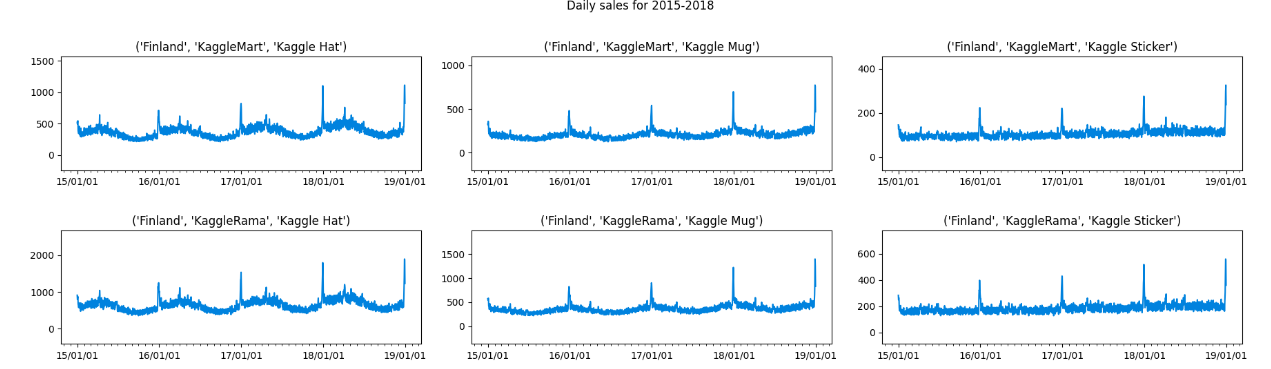
\includegraphics[scale=0.8]{02.png}
    \item
    At the same time, view the monthly sales figure.
    \\
    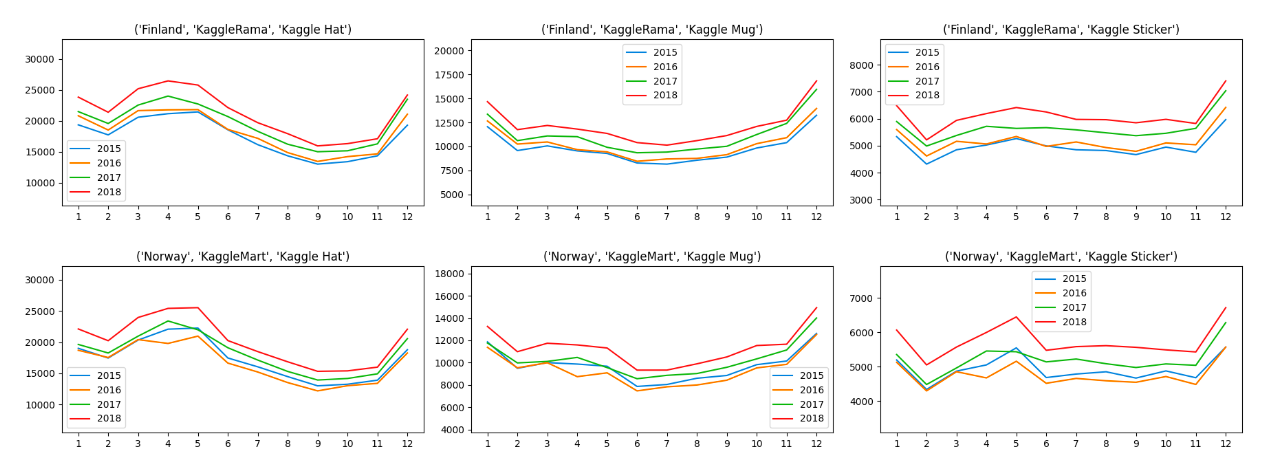
\includegraphics[scale=0.8]{04.png}
    \item
    View daily sales of the week.
    \\
    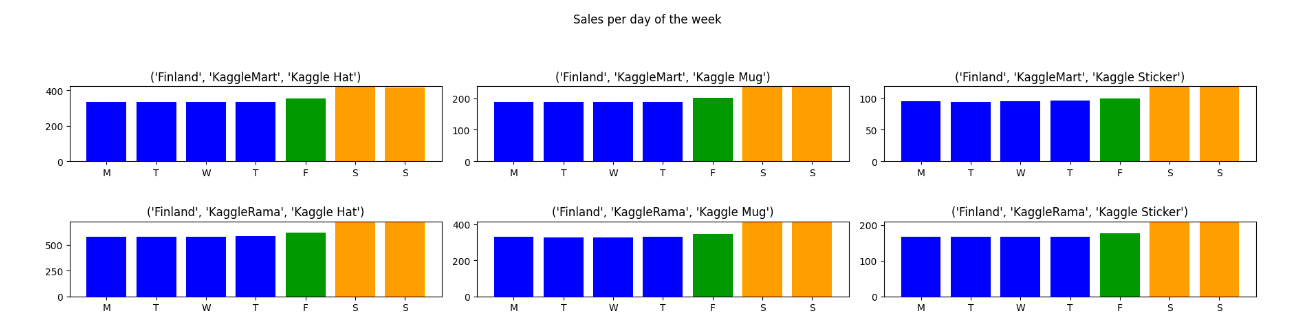
\includegraphics[scale=0.8]{03.png}
\end{itemize}


}
%%%%%%%%%% -------------------------------------------------------------------- %%%%%%%%%%


%%%%%%%%%% -------------------------------------------------------------------- %%%%%%%%%%

%\note{Note with default behavior}

%\note[targetoffsetx=12cm, targetoffsety=-1cm, angle=20, rotate=25]
%{Note \\ offset and rotated}

 % First column - second block


%%%%%%%%%% -------------------------------------------------------------------- %%%%%%%%%%

%%%%%%%%%% -------------------------------------------------------------------- %%%%%%%%%%


% SECOND column
\column{0.5}
 %Second column with first block's top edge aligned with with previous column's top.

%%%%%%%%%% -------------------------------------------------------------------- %%%%%%%%%%
\block{Data Processing}{
\begin{itemize}
	\item
	%\emph{Group Outlying Aspects Mining}
	Use Pandas database to operate the data, add GDP information, and add seasonal indicators every week. Unique coding for commodities, countries and stores. At the same time, Fourier feature is added.
	\\
	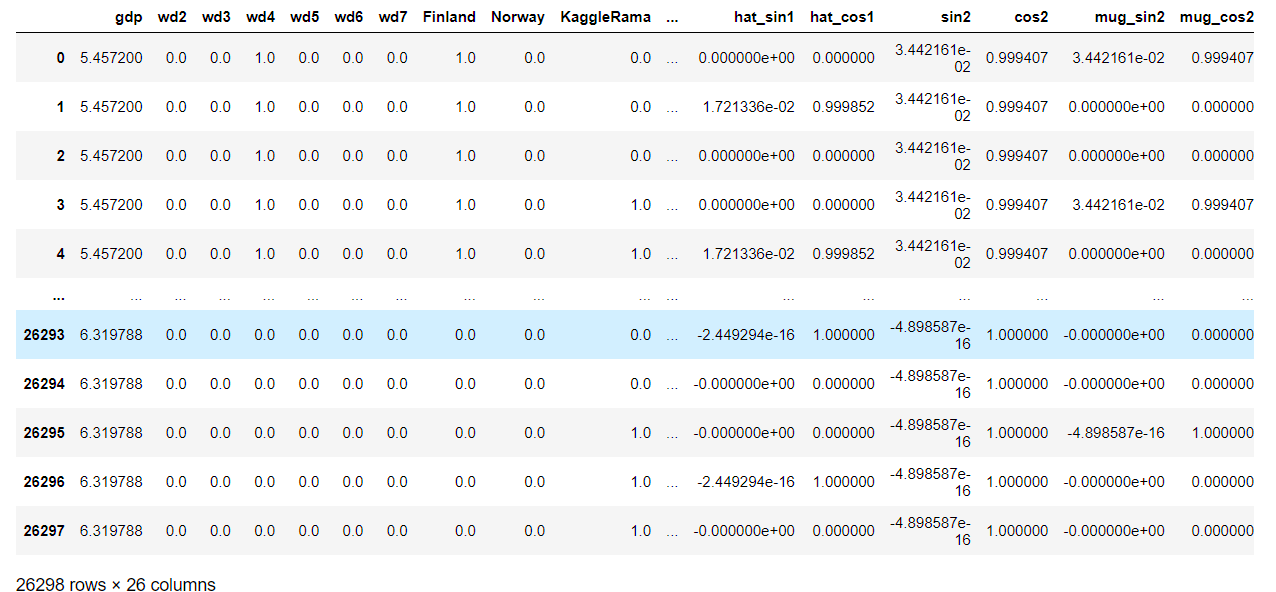
\includegraphics[scale=0.8]{07.png}

\end{itemize}
}
%%%%%%%%%% -------------------------------------------------------------------- %%%%%%%%%%
% Second column - first block


%%%%%%%%%% -------------------------------------------------------------------- %%%%%%%%%%
\block[titleleft]{Modeling and Result}
{
\item
  	Models: linear regression
  	\item
  	Public score: 6.48662
  	\item
  	Rank: 498/1543
}
%%%%%%%%%% -------------------------------------------------------------------- %%%%%%%%%%


% Second column - second block
%%%%%%%%%% -------------------------------------------------------------------- %%%%%%%%%%
\block[titlewidthscale=1, bodywidthscale=1]
{Conclusion}
{
\begin{description}
  The data structure is relatively simple, so the linear regression model is used for prediction. It is found that the loss value has relatively large deviation at some points, which may be related to the Spring Festival.
\end{description}
}
%%%%%%%%%% -------------------------------------------------------------------- %%%%%%%%%%


% Bottomblock
%%%%%%%%%% -------------------------------------------------------------------- %%%%%%%%%%
\colorlet{notebgcolor}{blue!20}
\colorlet{notefrcolor}{blue!20}


%\note[targetoffsetx=8cm, targetoffsety=-10cm,rotate=0,angle=180,radius=8cm,width=.46\textwidth,innersep=.1cm]{
%Acknowledgement
%}

%\block[titlewidthscale=0.9, bodywidthscale=0.9]
%{Acknowledgement}{
%}
%%%%%%%%%% -------------------------------------------------------------------- %%%%%%%%%%

\end{columns}


%%%%%%%%%% -------------------------------------------------------------------- %%%%%%%%%%
%[titleleft, titleoffsetx=2em, titleoffsety=1em, bodyoffsetx=2em,%
%roundedcorners=10, linewidth=0mm, titlewidthscale=0.7,%
%bodywidthscale=0.9, titlecenter]


%%%%%%%%%% -------------------------------------------------------------------- %%%%%%%%%%


\end{document}

%\endinput
%%
%% End of file `tikzposter-template.tex'.
